%\chaptermark{}ter{Finding low--energy spectrum of spin glass using CUDA}
\chapter[Brute--forcing spin--glass problems]{Brute--forcing spin--glass problems with CUDA}
\label{chapter:bruteforce}
Optimization problems play an important role in modern society, especially in current volatile times. Instances of such problems can be found in numerous areas of industry and applied sciences. One could mention logistic issues, such as vehicle routing problem together with its variants, and the famous protein folding problem or job shop scheduling to name just a few. It is often the case where many of the aforementioned problems fall into the so called NP--hard complexity class. This fact alone renders hard to solve, making the entire operational research a challenging endeavour requiring enormous amount of computational resources.

One way to tackle optimization problems is an exhaustive search over all possible solutions. Unfortunately, such brute--force approach quickly becomes impractical, as the number of possible solutions increases exponentially with the problem size. Nevertheless, despite its simplicity and obvious limitations, the brute--force algorithm is often the only approach capable of solving and certifying~\footnote{(i.e., proving that the found solution is in fact optimal)} \textit{arbitrary} problem instances within a given complexity class. For this very reason, efficient brute--force solvers are still considered to be an irreplaceable tool for testing and benchmarking other, often way more sophisticated, algorithms.

In this chapter, we demonstrate how the present--day, massively parallel, architectures can greatly increased attainable problem sizes of arbitrary Ising spin--glass instances that can be solved via exhaustive search. To this end, we harness the Nvidia CUDA technology  to find the low energy spectrum of the Ising Hamiltonian. The algorithm that we put forward allows one to search the solution space consisting of $2^{50}$ states in a reasonable time on, already on commodity hardware.

\section{Bruteforcing spin-glass problem using CUDA}
\subsection{Outline of the algorithm}
As already outlined in the introduction to this chapter, the idea of our algorithm is to visit each of the possible states of the system, compute its energy and choose desired number of lowest-energy states. Computing energy of multiple states is, quite obviously, an embarassingly parallel task, as energy of one state does not depend on the energies of other states.
Nevertheless, efficient implementation of exhaustive search poses several challenges, especially when done for massively parallel architectures.

In the ideal case of unlimited number of computation units\footnote{CPU cores or GPU threads} and memory, one could assign to each unit a task of computing energy of single state and then choose the desired number of lowest-energy states e.g. by sorting them in ascending order. However, in any real world system resources are limited, and such an approach quickly becomes impractical even for moderately-sized systems --- mainly because of an enormous amount of space needed for storing all of the possible states and energies.

One can overcome the above obstacle by observing that finding only $S$ lowest-energy states does not require knowledge of the whole spectrum at once.
To illustrate, if $S=1$ one could iterate over all possible states one-by-one, keeping global record of lowest-energy states found so far and updating this information whenever lower-energy solution has been found. Similarly, for arbitrary $S > 1$ one could iterate over possible solutions considering only a chunk of $k > S$ states at once, choose lowest $S$ states in the current chunk and then merge this information with the global record.

\todo[inline]{At this point it might be good to insert a pseucodoce.}

\subsection{Conversion to QUBO and computation of energy}
By performing a linear change of variables $s_i \mapsto 2q_i-1$ in spinglass problem, one obtains so called Quadratic Unconstrained Binary Optimization (QUBO) problem. Then, the function to be minimized takes a form
\begin{equation}
\label{eq:qubo2}
    F(q_1, \ldots, q_N) = \sum_{i=1}^N b_iq_i + \sum_{i \ne j} a_{ij} q_i q_j,
\end{equation}
where coefficients $b_i$ and $a_{ij}$ are given by
\begin{equation}
\label{eq:toQUBO2}
a_{ij}= 4J_{ij},
\quad 
b_i= 2h_i - 2 \sum_{\langle i, j \rangle} J_{ij}.
\end{equation}
and $F$ differs from $H$ by the constant offset $\sum_{i=1}^N h_i - \sum_{\langle i, j \rangle} J_{ij}$.

The two problems are clearly equivalent, however the QUBO formulation can be used to greatly accelerate computation of system energy. Indeed, one can factor out $q_i$ in \eqref{eq:qubo} and write $F$ in the following way.
\begin{equation}
    F(q_1, \ldots, q_N) = -\sum_{i=1}q_i \left(b_i + \sum_{j\ne i} a_{ij} q_j \right).
\end{equation}
Now, if given $q_i$ vanishes, then so does the whole $i$-th term of the outer sum. Therefore, the whole expression in the parenthesis does not have to be evaluated. Since each of $q_i$ vanishes exactly for half of all the possible system states, it follows that this simple optimization saves overall half of the multiplications done in the whole exhaustive search.

\subsection{Storage and representation of system states}
Implementing efficient algorithms involves choosing the right storage strategy for the data the algorithm operates on. This is especially the case for present-day GPUs. Indeed, graphic cards are equipped with fairly limited memory, as compared to operating memory available to the traditional CPU. Moreover, memory transfers between host and GPU induce additional overhead that should be avoided whenever possible. For this reason one often aims for designing storage strategy such that it reuses information already available on the GPU as much as possible, thus optimizing resource usage and minimizing number of memory transfers.

In principle, each state of the system can be represented by $N$ integers. However, since each variable can be assigned only one of two possible values, this wastes \emph{a lot} of available memory, as out of each machine word only a single bit is used. Instead, one can pack the whole state of the system into a single integer by identifying each bit of the underlying machine word with a single spin. 

Identifying states with integers greatly simplifies their enumeration, as it boils down to iterating over appropriate range of natural numbers. More importantly, it allows GPU threads to identify the system state they have to process using their index. The precise description of GPU scheduling is given in the next section.

\subsection{Implementation details}
\subsubsection{GPU scheduling}
In our implementation of the algorithm, each of the GPU thread computes energy of a single state. For a grid consisting of $2^N$ threads, the state given thread processes is given by a simple formula
\begin{equation}
\label{eq:state-to-thread-idx}
    \mathbf{q} = (\mbox{GPU thread index})_2
\end{equation}
Where $(n)_2$ denotes binary representation of integer $n$. In the case when algorithm has to be executed in chunks, equation \eqref{eq:state-to-thread-idx} has to be modified so that different states are processed in pass. Therefore, in general, the state being processed by the given thread is computed as
\begin{equation}
\mathbf{q} = ((\mbox{GPU thread index} + \mbox{chunk offset})_2
\end{equation}
where chunk offset for $i$-th chunk of size $2^l$ is simply $i2^l$.

\section{Improving the algorithm using Gray Code}

The algorithm presented in the previous chapter and its GPU--enabled implementation are already highly performant. However, we can still improve upon it by altering the order in which we enumerate the integral representation of states used by our algorithm.

\subsection{Single bit--energy difference}
Suppose we are given a QUBO with $F(q_{1},\ldots,q_{N})$ as in the equation \ref{eq:qubo}. Consider two states, say $\bq{1} = (\q{1}_{1},\ldots,\q{1}_{N})$ and $\bq{2}=(\q{2}_{1},\ldots,\q{2}_{N})$ such that they only differ in the $k$-th bit, i.e. $\q{2}_{k}=1-\q{1}_{k}$ and $\q{2}_{i}=\q{1}_{i}$ for $i \ne k$.
The energy difference $F(\bq{2})-F(\bq{1})$ can be easily computed and reads
\begin{align}
\begin{split}
  \label{eq:energydiff1}
  F(\bq{2})-F(\bq{1}) &= b_{k}(\q{2}_{k}-\q{1}_{k}) + \sum_{i\ne k}a_{ik}\q{1}_{i}(\q{2}_{k} - \q{1}_{k}) \\
                      &= (\q{2}_{k}-\q{1}_{k}) \left(b_{1} + \sum_{i \ne k}a_{ik}\q{1}_{i}\right) \\
  & = (1-2\q{1}_{k}) \left(b_{k} + \sum_{i \ne k}a_{ik}\q{1}_{i}\right).
\end{split}
\end{align}
Interestingly, computing the difference in equation \eqref{eq:energydiff1} requires only $N$ multiplications.   But how can this be used to improve the performance of the exhaustive search through QUBO state space?

Moving $F(\bq{1})$ to the right-hand side, we obtain a formula for $F(\bq{2})$ which requires only $N$ instead of maximum of $N(N+1)/2$ multiplications. Remember that this is only possible because $\bq{1}$ and $\bq{2}$ differ only by a single bit. If we could enumerate states in such a fashion that every consecutive two states differ only by a single bit, we could leverage the above formula instead of recomputing energy for each state from scratch. Before describing the algorithm, let us first introduce a notation that we will use later in this section. Given a state $\mathbf{q} = (q_{1},\ldots,q_{N})$, by $\flip{\mathbf{q}}{k}$ we will denote  a state resulting from flipping $k$-th bit of $\mathbf{q}$, i.e.
\begin{equation}
  \flip{\mathbf{q}}{k} \coloneq (q_{1}, \ldots, q_{k-1}, 1-q_{k}, q_{k+1}, \ldots, q_{N})
\end{equation}
and by $\diff_{F}(\mathbf{q},k)$ we will denote the difference between the energies of $\flip{\mathbf{q}}{k}$ and $\mathbf{q}$. Using the equation \eqref{eq:energydiff1}, we see that the expression for $\diff_{F}(\mathbf{q},k)$ is
\begin{align}
  \begin{split}
    \diff_{F}(\mathbf{q},k) = F(\flip{\mathbf{q}}{k}) - F(\mathbf{q}).
  \end{split}
\end{align}
The pseudocode for a serial algorithm for solving QUBO problem using our observations is outlined in listing \ref{lst:grayserial}. Before we can implement it on GPU though, we need two additional things:
\begin{enumerate}
  \item Producing sequence of bit flips that results in visiting all states.
  \item Strategy for dividing work among CUDA threads.
  \item Suitable modifications enabling us to use the algorithm to find the low energy-spectrum.
\end{enumerate}
We will first tackle the bit flipping problem. To compute the needed sequence of bit flips, we will use \emph{Gray code}, which we will describe now.
\begin{lstlisting}[
  language=Python,
  caption={Pseudocode for algorithm solving the QUBO problem using energy differences and bit flips.},
  captionpos=b,
  label=lst:grayserial,
  float,
  floatplacement=H
]
def solve_qubo(F, q):
    q = [0] * N # Start with all bits set to 0
    best_state = current_state = q
    best_energy = current_energy = F(q)

    for i in range(2 ** N - 1):
        k = find_next_bit_to_flip(q, i)
        current_energy = current_energy + diff(q, k)
        current_state = flip(q, k)
        if current_energy < best_energy:
            best_energy = current_energy
            best_state = current_state
    return best_state, best_energy
\end{lstlisting}
\subsection{Gray code}
When one talks about a binary encoding of integers, the first thing that comes to mind is a usual positional base-2 system. This encoding certainly does not fit our purpose.
Indeed, suppose $N=3$ and we are currently processing state corresponding to number $3$, whose representation in binary is $(011)_{2}$. The next state, corresponding to $4$ is encoded by the string $(100)_{2}$, which differs in all three bits.

Instead of using the positional system, we might utilize an encoding called Gray Code, or Reflected Binary Code (RBC), which is primarily used to improve the robustness of electromechanical switches and in error correction protocols. In this code, encoding of two successive integers always differs by at most one bit, which makes it suitable for application in our algorithm.

The conceptual construction of Gray Code is straightforward. For Gray Code of length $1$ we have two binary strings: $0$ and $1$. To obtain all Gray Codes for a given length $N > 1$, we first construct an ordered list of codes of length $N-1$ and call it $L$. Then, we reverse the list of codes, and call it $H$, an operation called \emph{reflection}. Finally, we prepend $0$ to all elements of $L$ and prepend $1$ to all elements of $H$. The concatenation of $L$ and $H$ forms the $N$--bit Gray Code. The process is illustrated in Fig. \ref{fig:gray} .One useful consequence of the construction is that the shorter Gray Codes might
be viewed as initial parts of the larger ones prepended with enough zeros. Thus,
statements as ``$n$-th Gray code'' make sense and are unambiguous.

\begin{figure}
  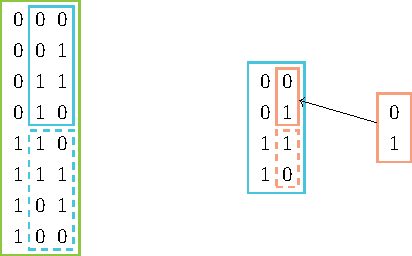
\includegraphics[width=\textwidth]{figures/gray.pdf}
  \caption{Reflection--based construction of Gray Code. The length of the code is denoted by $N$. For $N=1$, the code comprises two binary strings, $0$ and $1$. To construct the code of length $N>1$, the code of length $N-1$ and its vertical reflection are stacked. Then, the first, unreflected half is prepended with $0$ while the second, reflected half is prepended with $1$.}
  \label{fig:gray}
\end{figure}

An important thing to observe is that in our algorithm we need at most two Gray Code--encoded numbers at the time to determine the bit to be flipped. The reflection--based construction outlined so far would require precomputing a large part (if not all) of the encodings at once. Considering the size of the state space, this is clearly infeasible. However, there is a

While the construction presented above is useful for explaining the concept of the Gray Code, it is not efficient enough to be used in an algorithm. More precisely, with this procedure, we would need to use.

\section{Numerical results}
In order to test the performance of our algorithm, we run extensive benchmarks using the following hardware:
%
\begin{itemize}
\item CPU:
\href{https://ark.intel.com/products/94456/Intel-Core-i7-6950X-Processor-Extreme-Edition-25M-Cache-up-to-3-50-GHz-}{$10$
Cores {\rmfamily Intel\textregistered} Core \textsuperscript{TM}i7-6950X};
%
\item GPU(1): \href{https://www.nvidia.com/en-us/geforce/products/10series/geforce-gtx-1080}{Nvidia GeForce GTX $1080$, $8$GB GDDR$5$ global memory, $2560$ CUDA Cores};
%
\item  GPU(2): \href{https://www.nvidia.com/en-us/titan/titan-v/}{Nvidia Titan V, $12$GB HBM$2$ global memory, $5120$ CUDA Cores}.
\end{itemize}

For conducting our benchmarks we generated $100$ spinglass instances for each $N=24, 26, \ldots, 30, 32$. Additionally we generated $100$ instances of size $N=40$ and single instances of sizes $N=48, 50$ that were feasible to solve with Titan V GPU. Coefficients of each spinglass were drawn randomly from uniform distributions on the intervals $[-2, 2]$ and $[-1, 1]$ for magnetic fields and couplings respectively. For each instance, we computed low energy spectrum of $S=100$ states with our algorithm. We used maximum chunk size of $2^{29}$ for Titan V and CPU and chunk size of $2^{27}$ for GTX 1080.

As already mentioned, larger instances $(N > 32)$ were solved only using Titan V GPU. For GTX 1080 and CPU implementation, the expected time to solve those instances was estimated based on the timings for smaller $N$. The results of our benchmarks are are presented in figure \todo{Add figure with results}.

\begin{figure}
    \centering
    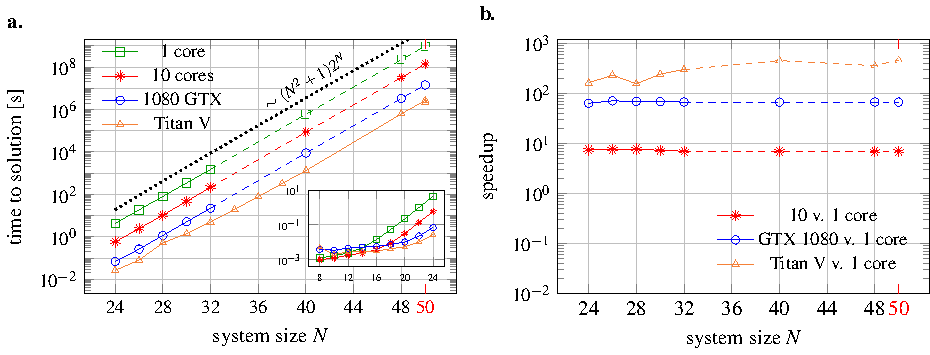
\includegraphics[width=\textwidth]{figures/resultsplot_reduced.pdf}
    \caption{Results of benchmarks of our algorithm. {\textbf{a.}} Time to solution vs. system size $N$. {\textbf{b.}} Speedup of multi-core/GPU implementation with respect to a single core one vs. system size $N$. The solid lines represent the numerical results and the dashed lines present estimates based on results obtained for smaller system sizes.}
    \label{fig:benchmark_results}
\end{figure}
%%% Local Variables:
%%% mode: latex
%%% TeX-master: "../main"
%%% End:
